\documentclass[11pt,a4paper,margin=0.5in]{report}

\usepackage[utf8]{inputenc}
\usepackage[francais]{babel}
\usepackage[margin=1in,footskip=0.25in]{geometry}
\usepackage{graphicx}
\usepackage[document]{ragged2e}
\usepackage{hyperref}

\title{IDF Eventer \\ UPMC M2 STL DAR Projet}
\author{Elias Boutaleb \\ Thierry Dondon}
\date{\today}

\begin{document}

\maketitle
\tableofcontents

\chapter{Introduction}

\section{Contexte}

IDF Eventer est une application réticulaire qui permet d'organiser des sorties dans l'Ile de France. \\
Ses utilisateurs peuvent au choix, soit voir des évènements qui leur sont intéressants et s'y inscrire, ou bien créer leurs propres évènements. \\
Pour l'instant, le choix d'évènements se limite à des sorties à pied ou à vélo.

\section{Fonctionnalités}

Un utilisateur a pour possibilité sur le site de :

\begin{itemize}
    \item S'inscrire et de se connecter à l'application
    \item Voir les derniers évènements
    \item S'inscrire à un évènement
    \item Voir ses inscriptions et les évènements qu'il organise
    \item Créer son propre évènement
    \item Commenter sur un évenement
\end{itemize}

\chapter{Manuel utilisateur}

\section{Description de l'interface}

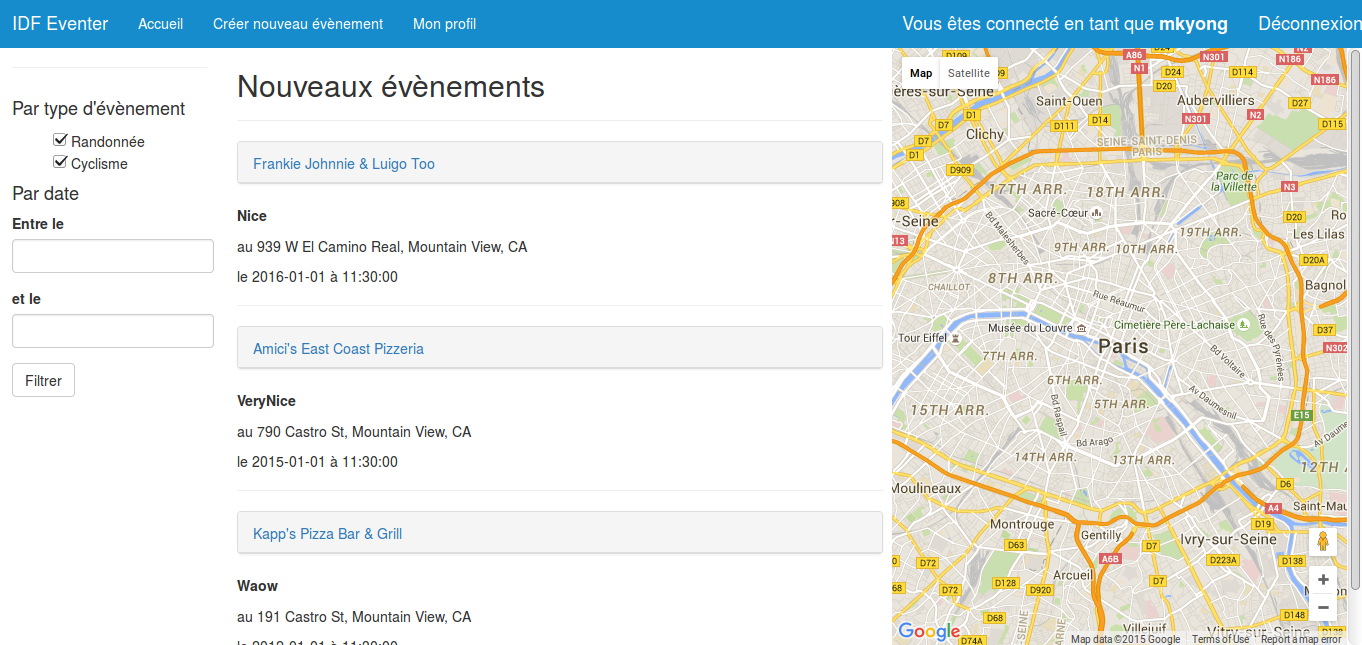
\includegraphics[scale=0.33]{illus/main.png}

Voici la page principale de l'application après connexion.\\
La barre de navigation permet respectivement d'accéder à la page ci-dessus, de créer un nouvel évènement, de consulter son profil et de se déconnecter
de l'application.\\

La barre latérale de gauche permet de filtrer selon critère les évènements affichés sur la carte sur la droite.\\
Au milieu, se trouvent les derniers évènements ajoutés par les autres utilisateurs. Ces derniers peuvent aussi être observés sur la carte.

\clearpage

\section{Cas d'utilisation}

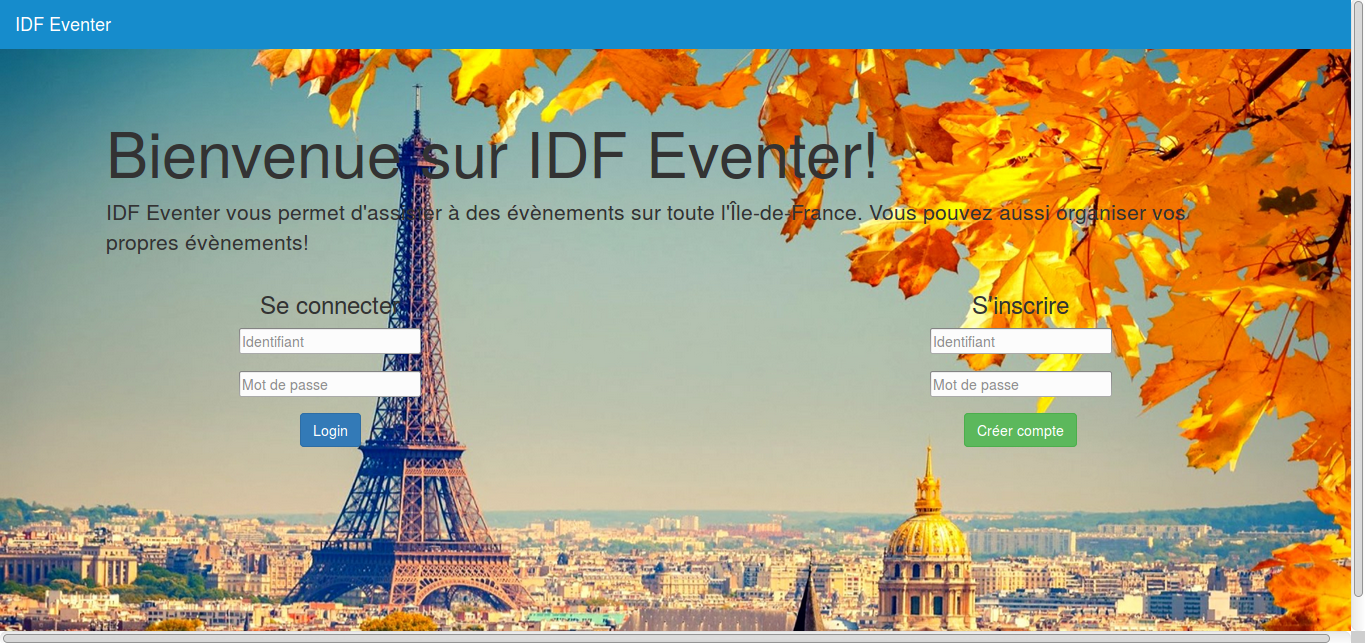
\includegraphics[scale=0.33]{illus/home.png} \\[0.25in]

Un nouvel utilisateur veut utiliser IDF Eventer; il s'inscrit en entrant un identifiant et un mot de passe de son choix. \\[0.25in]

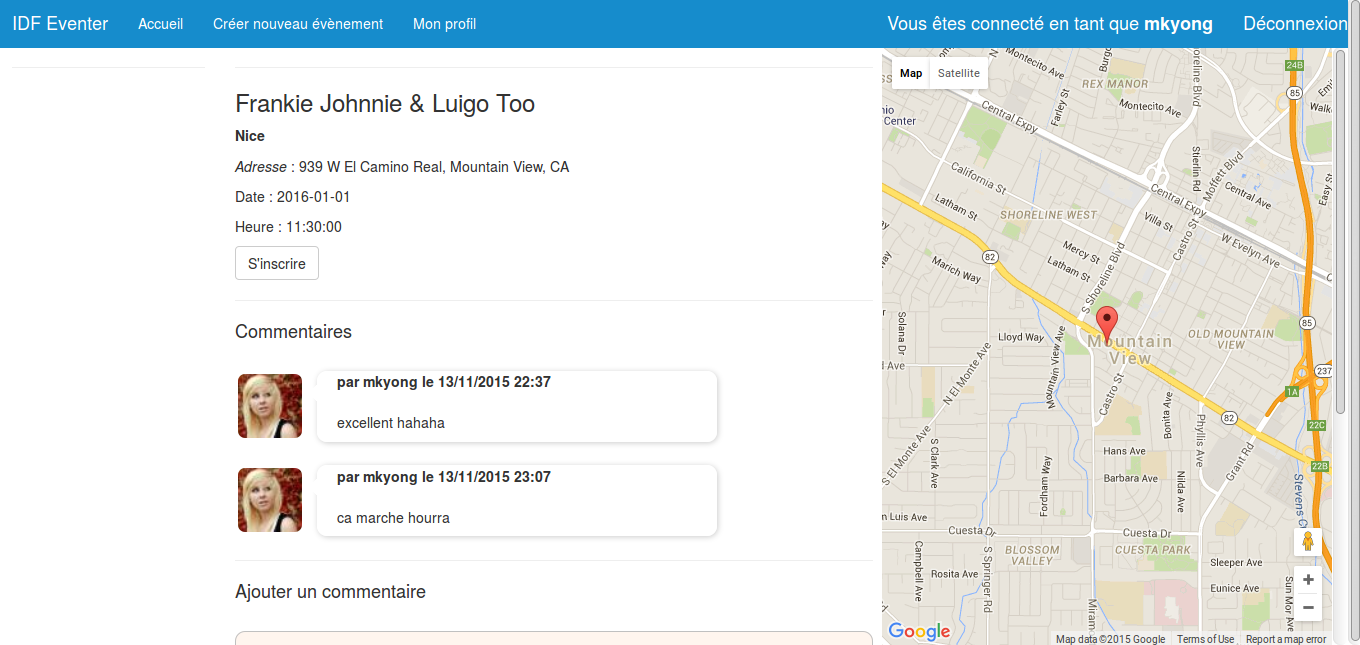
\includegraphics[scale=0.33]{illus/event.png} \\[0.25in]
Il arrive sur la page principale de l'application, et se trouve interessé par le dernier évenement ajouté en date. Il se rend donc sur la page de l'évènement. \\

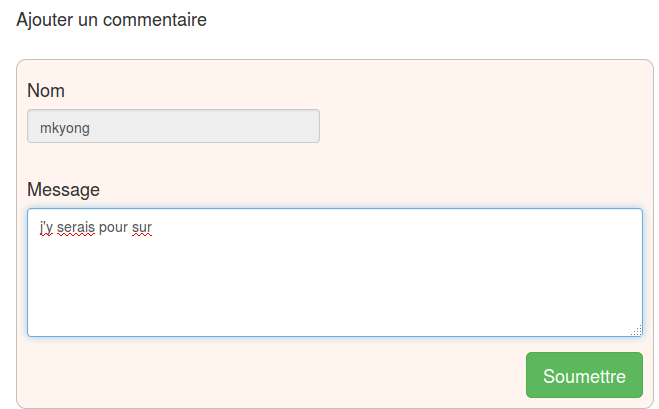
\includegraphics[scale=0.5]{illus/comment.png} \\[0.25in]
Il rédige un commentaire pour manifester son intérêt pour la sortie. \\[0.25in]

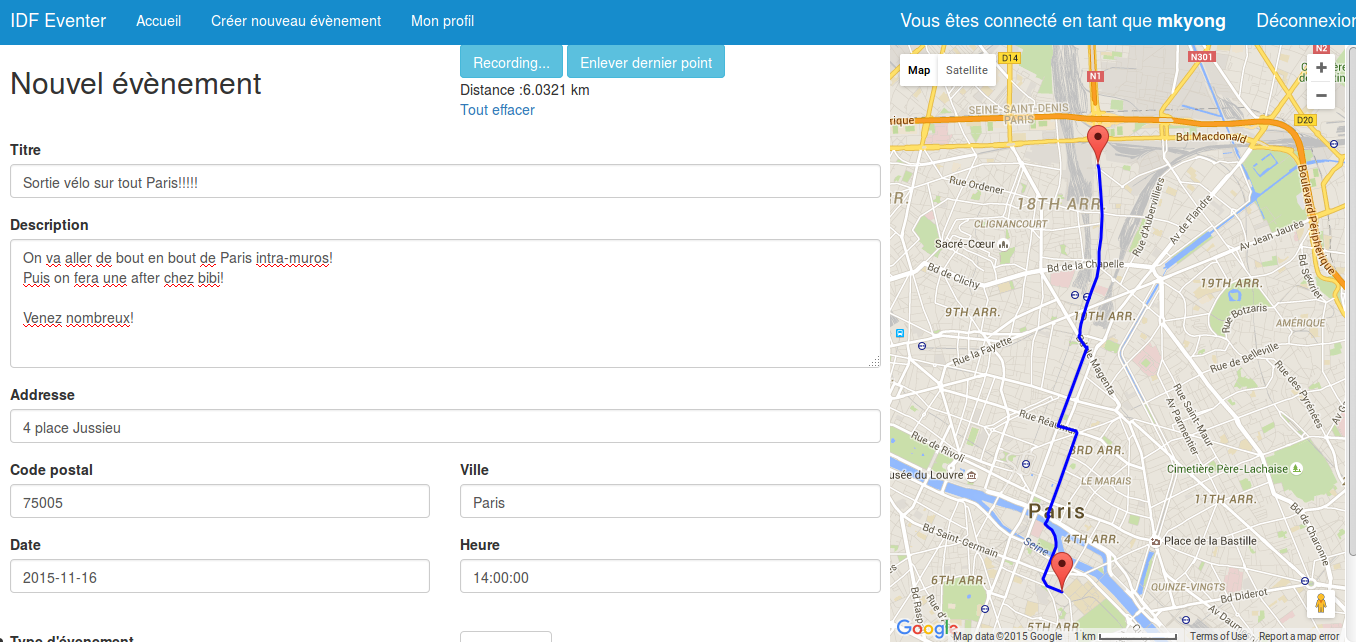
\includegraphics[scale=0.33]{illus/neweventroute.png} \\[0.25in]
Il réalise ensuite que la Californie est plutôt loin de la France, et décide de créer sa propre sortie en vélo sur Paris. \\[0.25in]

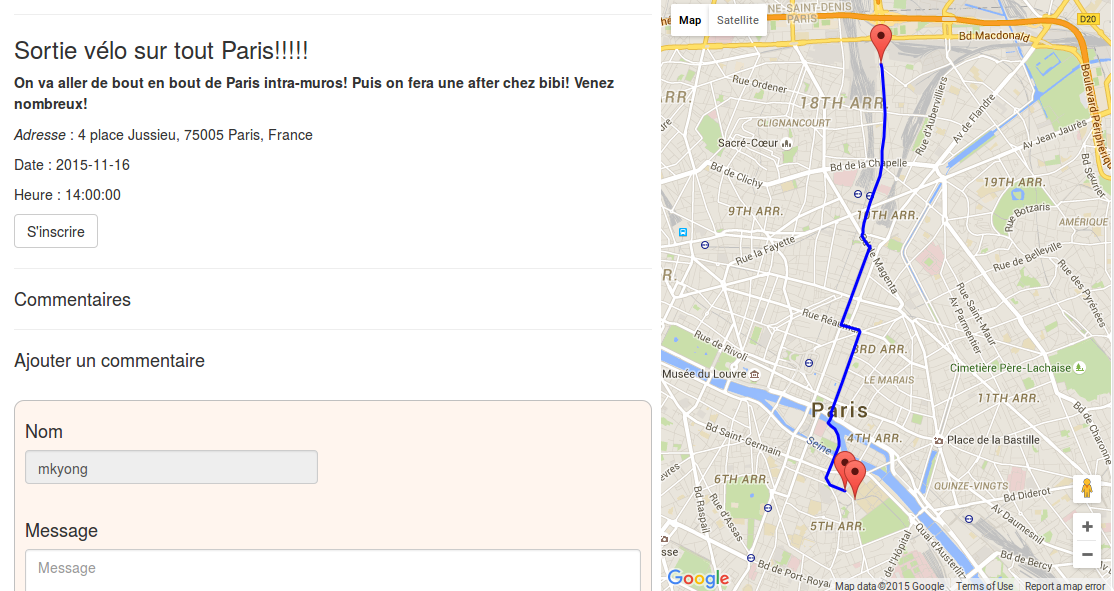
\includegraphics[scale=0.4]{illus/newev.png} \\[0.25in]
La page de la sortie après création. \\[0.25in]

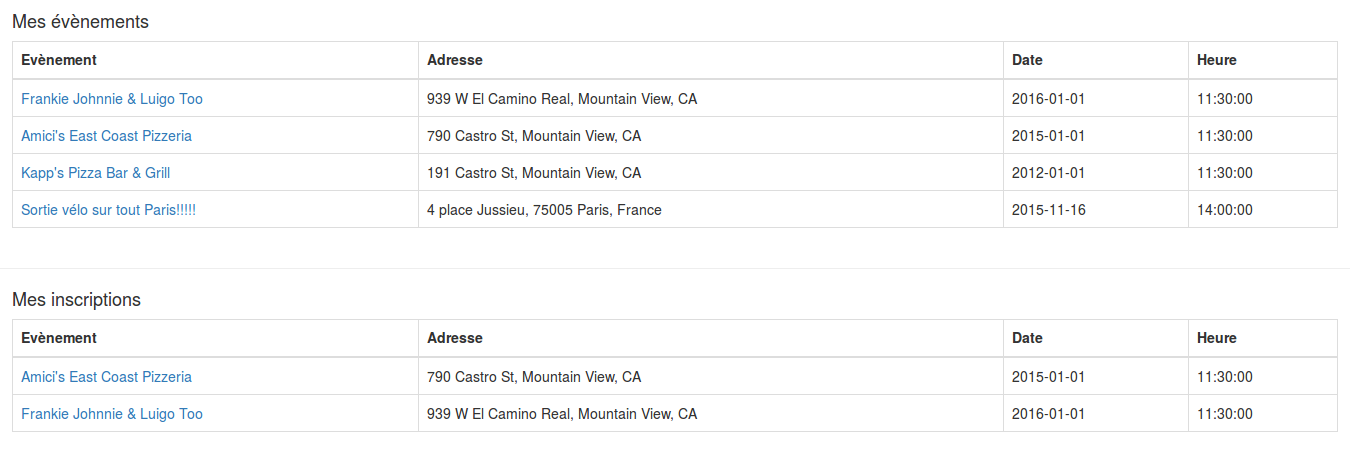
\includegraphics[scale=0.33]{illus/prof.png} \\[0.25in]
Il se rend ensuite sur son profil, pour voir ses sorties. \\[0.25in]

\chapter{Architecture de l'application}

\section{Schéma}

\begin{center}
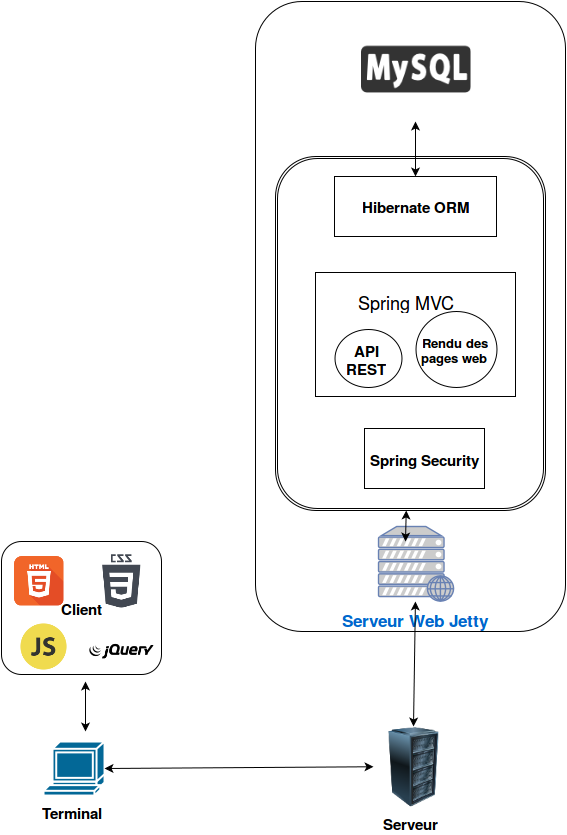
\includegraphics[scale=0.5]{illus/appschema.png} \\[0.25in]
\end{center}


\clearpage

\section{Choix techniques}

L'application côté serveur a été développée en Java, avec l'aide de plusieurs composants et librairies logicielles :

\begin{itemize}
    \item Jetty est un serveur Web HTTP. Il peut contenir des servlets, et d'autres applications peuvent y être adjoints si nécessaire. 
    \item Spring MVC Framework est un framework de développement d'application web.
    \item Spring Security est un module de connexion et d'authentification reposant sur Spring. 
    \item Hibernate est un framework qui permet de relier des objets Java à des n-uplets dans des tables d'une base de données relationelle.
    \item MySQL est une base de données relationelle utilisée pour lire et stocker les données traitées.
\end{itemize}

\vspace{0.5cm}

Les composants sélectionnés sont plutôt bien répandus dans les milieux de développement Java, 
par conséquent il est facile de trouver de la documentation concernant les fonctionnalités que nous avons choisi d'implémenter.\\[0.1in]

Le serveur génere des pages HTML à partir de pages Java Server (JSP), qui sont servies avec le code client en JavaScript et les feuilles de style CSS.\\[0.1in]
Le client communique avec l'application par le biais d'appels AJAX, et gère le rendu des informations avec jQuery.\\[0.1in]
Le rendu est géré avec Twitter Bootstrap.\\[0.1in]
La gestion des dates et de l'heure est supportée grâce à jQuery UI et le module TimeEntry\footnote{\url{http://www.keith-wood.name/timeEntry.html}}.\\[0.1in]
La manipulation des cartes se fait avec l'aide de l'API Google Maps.

\chapter{Extensions et améliorations}

\section{Avantages de l'application}
\begin{enumerate}
    \item Elle est extensible, grâce à l'architecture MVC qui rend facile l'ajout de nouvelles pages et des routes URL correspondantes.
    \begin{itemize}
        \item D'autres services peuvent être ajoutés dans leur propre conteneur Web grâce à Jetty.
    \end{itemize}
    \item Elle est facilement déployable grâce à Maven.
    \item L'utilisation d'Hibernate permet de prévenir les injections SQL.
    \item Si la création de clients pour d'autres plateformes est envisagée, il n'y a pas besoin de modifier le backend. Les clients pourront communiquer via l'API REST.
\end{enumerate}

\section{Inconvénients de l'application}
\begin{enumerate}
    \item Elle conserve les fichiers de configuration XML d'une archive Web (WAR), ce qui n'est pas toujours pratique.
    \item Elle repose beaucoup sur le client JavaScript pour le traitement préalable des données à envoyer au serveur et leur rendu sur les pages HTML.
    \item Elle a un mauvais rendu sur mobile, malgré le fait que le client utilise Bootstrap.
    \item Il n'y a pas eu d'étude de la sécurité de l'application.
        \begin{itemize}
            \item La validation des données aussi bien côté serveur que client est fragmentaire. 
            \item Laisser des champs vides ou y inserer du code HTML peut poser problème.
        \end{itemize}
    \item L'application n'est déployable pour l'instant que sur un système de type UNIX, mais pourrait tourner sur Windows avec des modifications mineures.
    \item Il faut être inscrit et connecté pour pouvoir profiter de l'application.
        \begin{itemize}
            \item Néanmoins, l'utilisation de l'API ne nécessite pas d'être authentifié. 
        \end{itemize}
\end{enumerate}

\section{Améliorations}
\begin{enumerate}
    \item Centraliser la configuration de Spring et Hibernate de manière programmatique permettrait de se passer des fichiers de configuration en XML.
    \item Améliorer le rendu sur tablettes et mobiles, rendre l'interface plus réactive.
    \item Renforcer la validation des données.
    \item Rendre l'application visible aux non-utilisateurs.
    \item Restreindre l'utilisation de l'API suivant les utilisateurs.
\end{enumerate}

\section{Extensions}
Les fonctionnalités suivantes pourraient être ajoutées à l'application:
\begin{enumerate}
    \item D'autres types d'évènements peuvent être gérés. (concerts, ateliers)
    \item Des lieux peuvent aussi y être répertoriés. (restaurants, lieux touristiques)
    \item Une option de recherche des évènements suivant des mots-clés.
\end{enumerate}

\end{document}
